%!TEX root = ../main.tex

\subsection{Synthetic Classification}\label{app:synthetic-classification}

\begin{figure}[t]
	\centering
    \ifdefined\smallPDF
	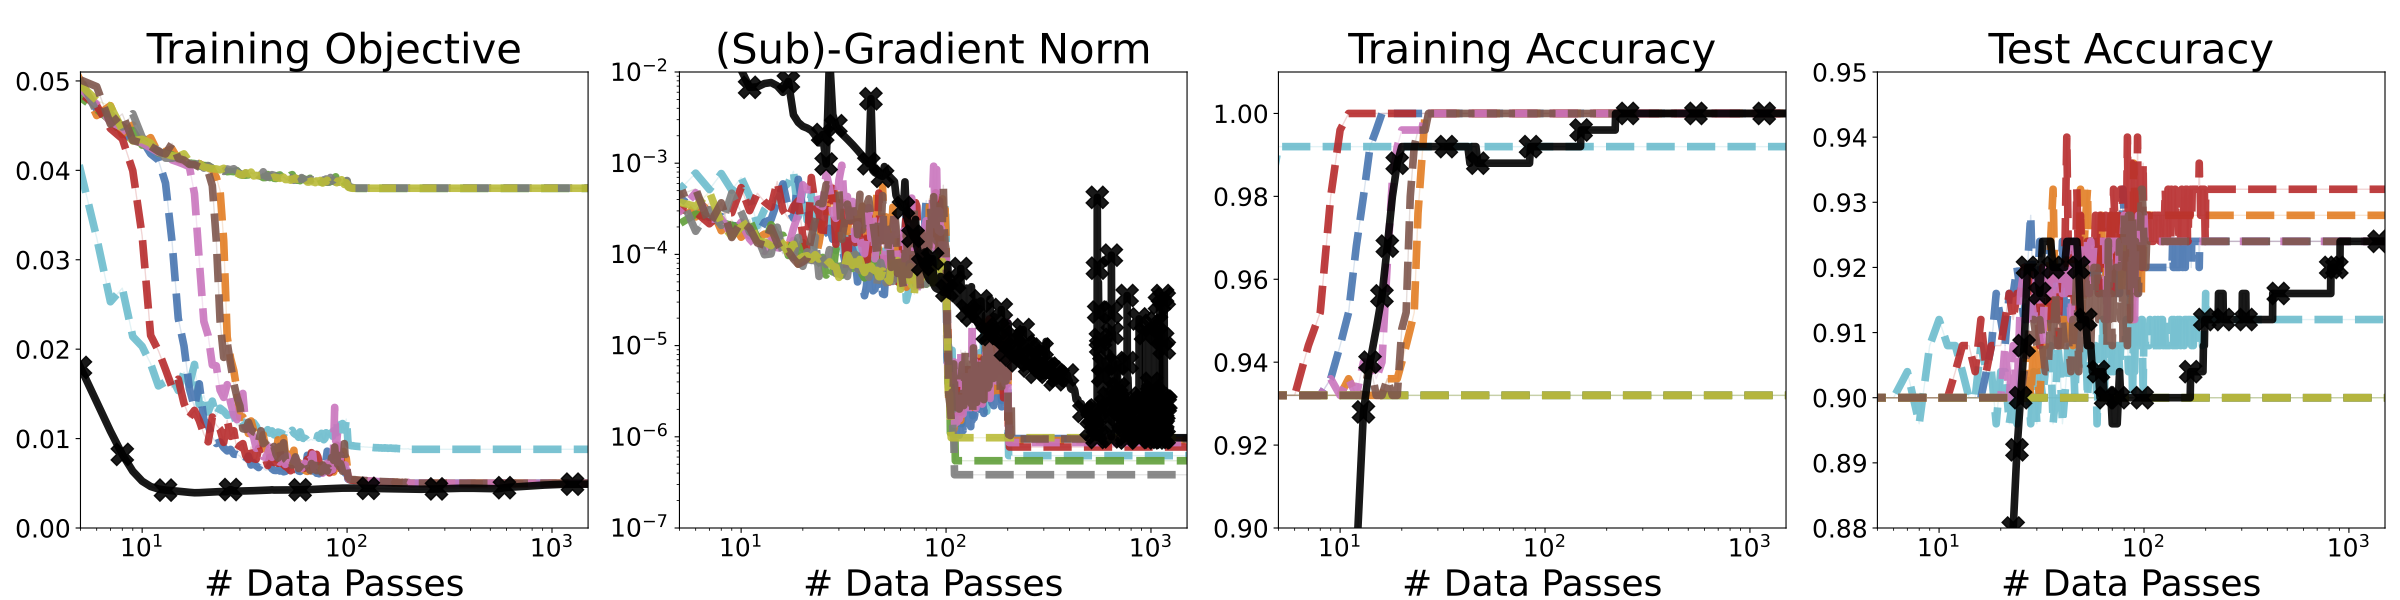
\includegraphics[width=0.98\linewidth]{figures/chapter_two/synthetic_classification_expanded.png}
    \else
	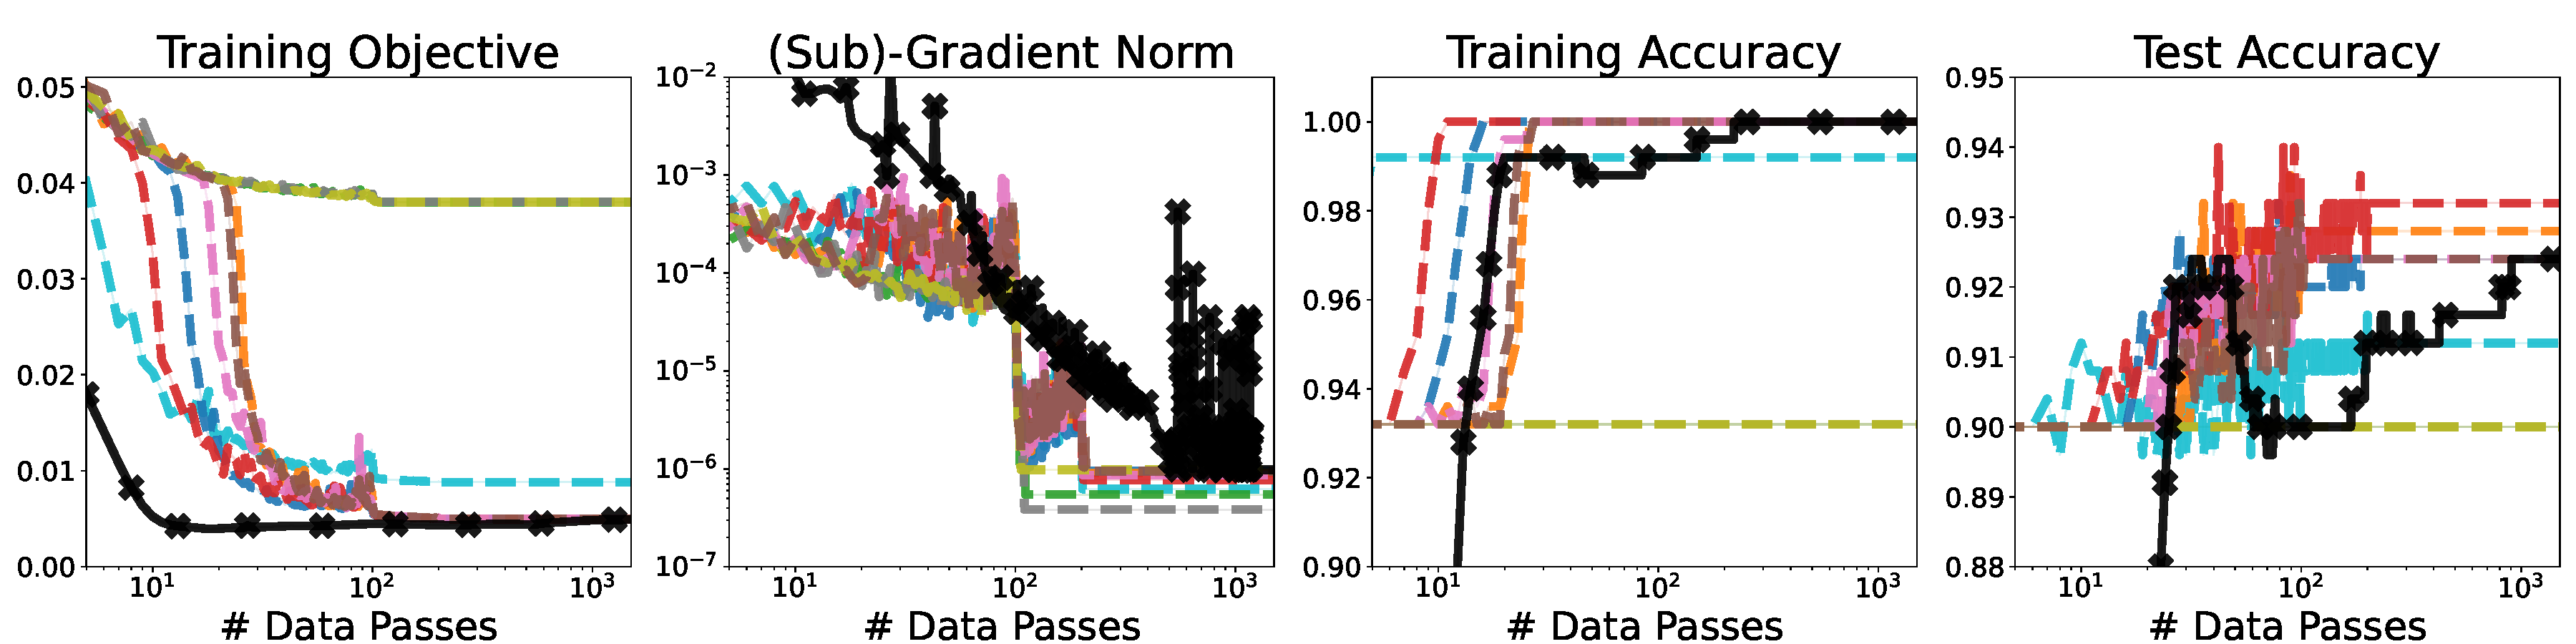
\includegraphics[width=0.98\linewidth]{figures/chapter_two/synthetic_classification_expanded.pdf}
    \fi
	\caption{Expanded version of \cref{fig:synthetic-classification} showing the square of the training gradient norm and test accuracy in addition to training objective and training accuracy, as reported in the main paper.
		Every run of SGD clearly converges to an approximate stationary point before terminating.
		The ``bumps'' in gradient norm for the AL method are caused by the dual updates, which increase the norm of the minim-norm subgradient of the augmented Lagrangian (\( \calL_\delta \)) with respect to the primal parameters.
	}%
	\label{fig:synthetic-classification-expanded}
\end{figure}

In this section, we provide additional details and results for the synthetic classification problem shown in \cref{fig:synthetic-classification}.

\textbf{Experimental Details}:
As mentioned in the main text, we generate the dataset by sampling \( X \sim \calN\rbr{0, \Sigma} \) and then taking \( y = \text{sign}(h_{W_1,w_2}(X)) \), where \( h_{W_1, w_2} \) is a two-layer ReLU network with \( m = 100 \) and random Gaussian weights.
We create \( 250 \) training examples and \( 250 \) test examples with \( d = 50 \) in this fashion.
The covariance matrix \( \Sigma \) is generated by sampling a random orthonormal matrix of eigenvectors and \( d - 2 \) eigenvalues from the interval \( [1, 10] \).
We then append \( 10 \) and \( 1 \) to this list and form \( \Sigma \) from the diagonalization;
this guarantees that the condition number of \( \Sigma \) is exactly \( 10 \).
Before optimization, we unitize the columns of the feature matrix (see Appendix~\ref{app:data-normalization}) to be consistent without our other experiments.

For the non-convex optimization problem, we use the standard PyTorch initialization and a step-size of \( 10 \).
This step-size gave the fastest convergence out of a grid of \( \{20, 10, 5, 1, 0.5, 0.1, 0.01\} \).
The mini-batch size is \( 25 \) examples (\( 10 \% \) of the dataset) and the maximum number of epochs is \( 1000 \).
We consider SGD to have converged when the gradient norm (as computed by PyTorch) is less than \( 10^{-3} \).
We change the global seed at each of the ten different runs, which ensures that both the initialization and mini-batch order/composition are different.
For our AL method, we randomly sample \( 100 \) ``diversity'' arrangements, which we augmented will activation patterns generated by SGD while optimizing the non-convex model.
Unlike SGD, the randomness in 10 runs of the AL method is due only to (i) sampling of the diversity set and (ii) the sign patterns from the SGD run.
Note that we are careful to use exactly the same runs of SGD as described above when using the active set method to compute \( \tilde \calD \).
We use the standard parameters as given in Appendix~\ref{app:default-parameters} for the remainder of the AL method's settings.

\textbf{Additional Results}:
\cref{fig:synthetic-classification-expanded} shows the convergence behavior of our AL and SGD.\@
As in the main paper, we omit all runs of the AL method but one because they are nearly identical.
One run of SGD diverges, while nine runs converge to stationary points as measured by the convergence criterion.
Of these, four converge to local minima with sub-optimal objective values; these models also do not have \( 100 \% \) accuracy on the training set despite the problem being realizable.
These sub-optimal local minimal also give worse test accuracy than the model found by the AL method.
